\documentclass[preprint,12pt]{elsarticle}

% --- Packages ---
\usepackage[utf8]{inputenc}
\usepackage[T1]{fontenc}
\usepackage{hyperref}
\usepackage{url}
\usepackage{booktabs}
\usepackage{amsfonts}
\usepackage{amsmath}
\usepackage{nicefrac}
\usepackage{microtype}
\usepackage{xcolor}
\usepackage{graphicx}
\usepackage{cleveref}
\usepackage{verbatim}
\usepackage{lineno}
\modulolinenumbers[5]

\journal{Journal of Molecular Graphics and Modelling}

\begin{document}

\begin{frontmatter}

\title{Differential Sensitivity to Semantic Perturbations in LLM-Based Molecular Property Prediction}

\author[inst1]{Muhammad Afif Erdita}
\ead{maeapip10@gmail.com}
\affiliation[inst1]{organization={SMA Negeri 23 Kabupaten Tangerang},
  city={Kabupaten Tangerang},
  state={Banten},
  postcode={15821},
  country={Indonesia}}

\begin{highlights}
\item Controlled perturbation framework isolates semantic effects in LLM predictions
\item Structural topic focus is associated with directional gain, not hallucination type
\item Task-dependent asymmetry: directional trends on BBBP, significant degradation on BACE
\item Random-permutation control separates semantic content from stylistic priming
\item Larger models show reversed sensitivity to semantic perturbations
\end{highlights}

\begin{abstract}
Recent studies suggest that large language model (LLM) hallucinations may influence molecular property prediction, yet the nature of this effect remains poorly characterized. We introduce a controlled semantic perturbation framework to evaluate how structured modifications --- which we characterize as synthetic semantic priors --- influence zero-shot prediction. We evaluate nine conditions on two MoleculeNet benchmarks (BBBP, $N=204$; BACE, $N=152$) using multi-seed evaluation (Llama-3.1-8B) and cross-model validation (Llama-3.3-70B). On BBBP, prompt-constrained structural augmentation (C4a) yields the largest observed ROC-AUC increase (0.626 vs. 0.533 baseline), although shifts were not statistically significant after correction ($p > 0.05$). Post-hoc verification suggests that the structural topic focus of the perturbation, rather than its factual accuracy, is the primary driver of performance shifts, as C4a outputs predominantly fall into contextual descriptions despite their structural focus. On BACE, we find robust and statistically significant performance degradation across nearly all hallucination conditions, ditandai oleh systematic ``distributional compression'' of predicted probabilities toward a non-discriminative low-confidence state. A random-permutation control confirms that observed effects are driven by semantic alignment rather than scientific register alone, suggesting a functional link between perturbation content and model response. These findings indicate that LLM-based molecular predictions exhibit differential sensitivity to structured semantic perturbations, highlighting the importance of controlled evaluation in scientific reasoning pipelines.

\end{abstract}

\begin{keyword}
large language models \sep molecular property prediction \sep 
hallucination \sep semantic perturbation \sep cheminformatics \sep 
zero-shot learning
\end{keyword}

\end{frontmatter}

\linenumbers

\section{Introduction}

Molecular property prediction is a critical component of early-stage drug discovery, enabling the prioritization of candidate compounds before expensive synthesis and biological assays~\cite{vamathevan2019applications}. Machine learning approaches---including graph neural networks~\cite{gilmer2017neural}, fingerprint-based classifiers~\cite{rogers2010extended}, and descriptor-based models---have become standard tools, with MoleculeNet~\cite{wu2018moleculenet} providing widely adopted benchmarks across physicochemical, enzymatic, and toxicity tasks.

More recently, large language models (LLMs) have been applied to molecular reasoning by converting SMILES notation into natural language contexts for text-based inference~\cite{guo2024llm, ross2022large}. Within this line of work, an observation has been reported in prior work: hallucinated molecular descriptions---scientifically styled but factually incorrect text---have been associated with improved downstream prediction performance in specific settings~\cite{hao2024hallucination}. This finding is in tension with the common assumption that strict factual correctness is a prerequisite for useful textual augmentation. We note that zero-shot LLM inference is not intended to replace specialized molecular prediction models; rather, the LLM serves as a controlled experimental substrate---a ``cognitive assay''---for investigating how semantic perturbations propagate through text-conditioned prediction pipelines.

However, existing investigations of this phenomenon share several limitations. First, hallucination is typically treated as a monolithic category, obscuring potentially important differences among types of factual error. Second, prior studies often lack semantic controls capable of disentangling the contribution of molecular-relevant content from generic scientific language effects (stylistic priming). Third, it remains unclear whether these hallucination-associated performance variations generalize across prediction tasks with different underlying knowledge requirements. Understanding this sensitivity is important for interpreting LLM-augmented predictions, particularly in settings where textual augmentation may introduce uncontrolled semantic perturbations.

The primary contribution of this work is the introduction of a controlled semantic perturbation framework to systematically evaluate how structured semantic alterations influence LLM-based molecular prediction. We define a lightweight, heuristic categorization scheme comprising three prompt-constrained perturbation operators---Structural Phantom (SP), Property Inversion (PI), and Mechanism Fabrication (MF)---alongside a residual Contextual Confabulation (CC) class. We note that these labels describe the \textit{prompt design intent}; as detailed in Section~\ref{sec:taxonomy}, the actual outputs may not conform to the intended taxonomy class. We evaluate this framework through a nine-condition ablation on two MoleculeNet benchmarks representing distinct regimes: BBBP (physicochemical) and BACE (enzyme inhibition).

Our key contributions include:
\begin{itemize}
    \item A controlled perturbation framework enabling the systematic isolation of hallucination-associated performance variations through semantic and stylistic disruption.
    \item A lightweight categorization scheme for molecular description errors, operationally defined as perturbation operators to maintain interpretability and reproducibility.
    \item A task-dependent divergence in semantic augmentation sensitivity: prompt-constrained structural augmentation (C4a) yields directional improvements on BBBP, while most hallucination conditions significantly degrade BACE performance. Post-hoc verification reveals 0\% SP classification for C4a, indicating that the prompt's structural topic focus---rather than hallucination type---underlies the observed effect.
    \item Characterization of prediction distribution compression on BACE, where hallucination augmentation shifts bimodal baseline distributions toward non-discriminative narrow peaks.
    \item A random-permutation control experiment establishing that semantic content, rather than stylistic register alone, is the primary contributor to observed performance shifts.
    \item Architecture-dependent hallucination sensitivity, where smaller models exhibit directional performance gains under hallucination augmentation on physicochemical tasks, while larger models show reversed sensitivity.
\end{itemize}

This exploratory study is bounded to two LLM scales and two datasets ($N=204$ for BBBP, $N=152$ for BACE). As a cognitive assay of semantic sensitivity, the findings are intended to structure future empirical investigation into LLM augmentation rather than to establish causal mechanisms.

\section{Related Work}
\label{sec:related_work}

\subsection{Molecular Property Prediction}
Molecular property prediction has been standardized through benchmark suites such as MoleculeNet~\cite{wu2018moleculenet}, which provides curated classification and regression tasks spanning physicochemical, biophysical, and physiological domains. State-of-the-art approaches include message-passing neural networks (MPNNs)~\cite{gilmer2017neural}, graph transformer architectures~\cite{ying2021transformers}, and descriptor-based models using extended-connectivity fingerprints~\cite{rogers2010extended}. Scaffold splitting~\cite{bemis1996properties} is widely adopted to evaluate generalization under structural novelty. \textbf{Distinction:} Our work is not a model development study. We do not propose a new prediction architecture. Rather, we use an existing LLM in a zero-shot setting to investigate how different types of textual augmentation affect prediction behavior.

\subsection{LLMs in Molecular Science}
Large language models have been increasingly applied to chemical tasks, including reaction prediction~\cite{schwaller2019molecular}, retrosynthesis~\cite{liu2024retrosynthesis}, and molecular property estimation~\cite{guo2024llm, ross2022large}. Text-based molecular representations, where SMILES strings are accompanied by natural language descriptions, have shown promise for zero-shot and few-shot inference~\cite{edwards2022text2mol}. Recent studies have explored whether LLMs encode implicit chemical knowledge through their pre-training corpora~\cite{white2023assessment}. \textbf{Distinction:} Our work is not a prompt engineering study. We do not optimize prompts for maximum prediction accuracy. Instead, we use a fixed prompt template to systematically vary the semantic content of augmentation text while controlling for confounding factors.

\subsection{Hallucination in Scientific LLM Applications}
LLM hallucination---the generation of fluent but factually unsupported text---has been extensively studied in general NLP contexts~\cite{ji2023survey, huang2023survey}. In molecular and scientific applications, hallucination poses particular risks because factual errors in structural or mechanistic claims may not be easily detected by non-expert users~\cite{ramos2024review}. Recent work by Hao et al.~\cite{hao2024hallucination} reported the counterintuitive finding that hallucinated descriptions can improve molecular property prediction, though without characterizing which aspects of the hallucinated text drive this effect. Yuan et al.~\cite{yuan2025taxonomy} proposed a taxonomy for molecular hallucinations but did not conduct controlled ablation experiments isolating the contribution of each category. \textbf{Distinction:} Our work is not a hallucination detection or mitigation study. We treat hallucinations as structured semantic perturbations and study their differential effects on prediction behavior through controlled ablation, incorporating semantic and stylistic controls absent from prior evaluations.

\section{Methods}
\label{sec:methods}

\subsection{Heuristic Categorization Scheme}
We utilize a heuristic categorization scheme to structure our analysis of natural molecular hallucinations (C3). Each type is detectable through rule-based classification using RDKit~\cite{landrum2023rdkit} as the ground-truth engine. We emphasize that this scheme is a heuristic tool, not an exhaustive semantic ontology. The keyword sets were intentionally constrained to maintain interpretability and reproducibility rather than maximize coverage. The categories are mutually exclusive and applied in priority order (SP $>$ PI $>$ MF $>$ CC):

\begin{itemize}
    \item \textbf{Structural Phantom (SP):} The generated text references chemical elements or functional groups that are absent from the molecular structure. Detection: for a predefined heuristic dictionary of element keywords (e.g., ``fluorine'', ``fluoro''), we check whether the corresponding element is present in the molecule's atom set via \texttt{mol.GetAtoms()}. If a keyword matches but the element is absent, the description is classified as SP.
    \item \textbf{Property Inversion (PI):} The generated text claims physicochemical properties that contradict computed descriptors. Detection: we compute MolLogP via RDKit. If LogP $> 3$ and the text contains keywords from a predefined hydrophilic dictionary, or LogP $< 1$ and the text contains keywords from a lipophilic dictionary, the description is classified as PI.
    \item \textbf{Mechanism Fabrication (MF):} The generated text names specific biological targets or pathways. Detection: exact keyword matching against a fixed list of 9 common targets (e.g., ACE2, HER2, EGFR).
    \item \textbf{Contextual Confabulation (CC):} The residual category. Descriptions that do not trigger SP, PI, or MF criteria are classified as CC. This category represents scientifically plausible but generic narrative hallucination.
\end{itemize}

We acknowledge that CC functions as a residual class and encompasses heterogeneous subtypes that future work should further differentiate.

\subsection{Experimental Conditions}
Our ablation framework consists of nine conditions, designed to isolate the contributions of semantic content, scientific register, and hallucination type:

\begin{itemize}
    \item \textbf{C0 (Baseline):} SMILES notation only, with no augmentation.
    \item \textbf{C1 (Factual):} SMILES augmented with a factual description generated by RDKit (molecular weight, LogP, hydrogen bond donors/acceptors, TPSA, ring count, atom composition).
    \item \textbf{C2 (Chemical Priming):} SMILES augmented with a template-generated text using scientific-sounding but semantically vacuous language that includes chemical vocabulary. We note that C2 is \emph{not} a pure stylistic control because it contains domain-relevant vocabulary; C2b serves as the stricter control.
    \item \textbf{C2b (Pure Gibberish):} SMILES augmented with template-generated text using exclusively non-chemical vocabulary. This condition strictly controls for prompt length and linguistic complexity without domain priming.
    \item \textbf{C3 (Free Hallucination):} SMILES augmented with an unconstrained LLM-generated description, replicating the protocol of prior work~\cite{chen2023llm4mol}.
    \item \textbf{C4a (Structural Augmentation):} SMILES augmented with text generated via prompt-constrained forcing to explicitly describe structural features and functional groups. We emphasize that C4a--c represent prompt-constrained semantic perturbations rather than naturally occurring hallucinations classified post-hoc. To validate this constraint, we applied the heuristic classifier to a representative sample of generated C4a descriptions ($n=49$). The results revealed a notable methodological limitation: 0\% of C4a outputs were classified as SP, and the vast majority defaulted to CC. This occurred because the LLM generated scientifically plausible structural descriptions (e.g., ``contains a benzene ring'') that do not reference absent elements---the specific criterion required by the SP heuristic (which checks for keywords like ``fluorine'' or ``chloro'' against the molecule's actual atom set). Consequently, the C4a--c conditions must be strictly interpreted as \textit{prompt-constrained semantic perturbations} (focusing the LLM on structural, property, or mechanism topics), rather than verified taxonomy classes.
    \item \textbf{C4b (Property Inversion):} SMILES augmented with text generated via prompt-constrained forcing to explicitly describe solubility, lipophilicity, and permeability.
    \item \textbf{C4c (Mechanism Fabrication):} SMILES augmented with text generated via prompt-constrained forcing to explicitly hypothesize biological targets and cellular mechanisms.
    \item \textbf{C5 (Random-Permutation):} SMILES augmented with a hallucination originally generated for a \emph{different} molecule, assigned via a fixed random permutation ($seed=42$). This preserves the scientific register and statistical properties of hallucinated text while completely disrupting semantic alignment with the target molecule.
\end{itemize}

\subsection{Prediction Protocol}
All prediction queries use a fixed zero-shot prompt template:

\begin{quote}
\texttt{Given this molecule (SMILES: \{smiles\})}\\
\texttt{[Additional information: \{augmentation\}]}\\
\texttt{On a scale of 0 to 1, what is the probability that this molecule can \{task\}?}\\
\texttt{Respond with ONLY a number between 0 and 1. Nothing else.}
\end{quote}

The augmentation line is omitted for C0. The task description is ``penetrate the blood-brain barrier'' for BBBP and ``inhibit the BACE-1 enzyme'' for BACE. For the extended generalization benchmarks, the task descriptions were: ``exhibit toxicity in the NR-AR assay'' for Tox21 (selected as a representative nuclear receptor assay to provide a mechanistic contrast to the enzymatic reasoning required for BACE), and ``provide a water solubility (logS) value consistent with the molecule's structure'' for ESOL. For ESOL, the task was framed as log-solubility regression; RMSE was calculated directly on the predicted numerical values extracted from LLM responses. All other prompt elements remained identical to the primary ablation. The numerical output was deterministically extracted, with malformed responses defaulting to 0.5 for classification tasks and 0.0 for regression.

\subsection{Implementation Details}
\label{sec:implementation}
\textbf{Model.} Primary ablation experiments were conducted with \texttt{Llama-\allowbreak 3.1-\allowbreak 8B-\allowbreak Instant} via the Groq API. Cross-model validation was extended to \texttt{Llama-\allowbreak 3.3-\allowbreak 70B-\allowbreak Versatile}, as described in Section~\ref{sec:implementation_robustness}.

\textbf{Generation parameters.} Prediction queries: temperature $= 0.0$, $\texttt{max\_tokens} = 10$, $\texttt{seed} = 42$. Hallucination generation: temperature $= 0.9$, $\texttt{max\_tokens} = 150$, no fixed seed. We explicitly distinguish between stochastic hallucination generation (no fixed seed) and quasi-deterministic prediction inference (seed=42), noting that API-level non-determinism may still introduce minor variability. To ensure exact reproducibility despite stochastic generation, the static dataset containing all generated augmentations used for evaluation is provided in the repository. Failed API calls (rate limits, parsing errors) defaulted to $p = 0.5$; the proportion of such defaults is reported in Appendix~\ref{subsec:api_failures}.

\textbf{Data.} Datasets were loaded via DeepChem~\cite{ramsundar2019deepchem}. Both BBBP ($N=204$) and BACE ($N=152$) were partitioned using scaffold splitting~\cite{bemis1996properties} via DeepChem's built-in splitter (80/10/10 train/valid/test). Only the held-out test set was used for evaluation.

\textbf{Factual descriptions.} For condition C1, factual descriptions were generated using RDKit molecular descriptors: molecular weight, Wildman-Crippen LogP, number of hydrogen bond donors and acceptors, topological polar surface area, heavy atom count, and ring count.

\textbf{Traditional ML Baseline.} To provide context for the zero-shot LLM predictions, we trained a Random Forest classifier (500 trees) using Morgan fingerprints (radius=2, 2048 bits) on the training and validation partitions of the scaffold split. The baseline was evaluated on the exact same test sets ($N=204$ for BBBP, $N=152$ for BACE) to ensure strict comparability.

\textbf{Extended Generalization Benchmarks.} To assess 
cross-task generalizability of the primary findings, a 
targeted subset of conditions---baseline (C0), free 
hallucination (C3), and prompt-constrained structural 
augmentation (C4a)---was evaluated on two additional 
MoleculeNet benchmarks: Tox21 (multi-task toxicity 
classification, evaluated on the first task column) and 
ESOL (aqueous solubility regression). These three 
conditions were selected to represent the no-augmentation 
reference, the maximal perturbation condition, and the 
best-performing augmentation identified in the primary 
ablation, respectively. Full nine-condition ablation on 
these datasets is reserved for future work given the 
exploratory scope of this study. Results are reported in 
Table~\ref{tab:generalization}.

\subsection{Evaluation and Calibration Metrics}
Discriminative performance was assessed using the area under the receiver operating characteristic curve (ROC-AUC). To account for the single-split evaluation, 95\% confidence intervals were computed via bootstrap resampling (1,000 iterations, seed $= 42$). 

To characterize the observed ``distributional compression'' and its impact on model reliability, we evaluate model calibration using the Brier score and Expected Calibration Error (ECE). The Brier score measures the mean squared difference between predicted probabilities ($f_i$) and actual outcomes ($y_i$):
\begin{equation}
BS = \frac{1}{N} \sum_{i=1}^{N} (f_i - y_i)^2
\end{equation}
ECE partitions the predicted probabilities into $M=10$ equally spaced bins ($B_m$) and computes the weighted average of the absolute difference between bin accuracy and bin confidence:
\begin{equation}
ECE = \sum_{m=1}^{M} \frac{|B_m|}{N} |acc(B_m) - conf(B_m)|
\end{equation}

Statistical significance for ROC-AUC differences relative to the baseline (C0) was assessed using a bootstrap paired difference test. Multiple comparisons were corrected using the Benjamini-Hochberg procedure (hereafter $p_{\text{BH}}$). We also report Cohen's $d$ on the raw prediction score distributions to quantify the shift in model confidence induced by semantic perturbations.

\subsection{Preliminary Scaling Exploration}
\label{sec:implementation_robustness}
To assess whether the observed phenomena persist across model scales, we performed two preliminary exploration steps:
\begin{enumerate}
    \item \textbf{Multi-Seed Stability (8B):} For the primary Llama-3.1-8B model, we repeated the prediction protocol for conditions C0 and C3 across three independent runs (seeds 42, 123, 777) to observe performance variance.
    \item \textbf{Pilot Scale Exploration (70B):} To observe behavior at a larger scale, we executed the prediction protocol for C0 and C3 on the \texttt{Llama-\allowbreak 3.3-\allowbreak 70B-\allowbreak Versatile} model.
\end{enumerate}
This exploration was designed to distinguish systematic semantic effects from model-specific quirks at the 8B scale.

\section{Results}
\label{sec:results}

\subsection{Predictive Performance Across Conditions}

Table~\ref{tab:results} and Figure~\ref{fig:performance} summarize ROC-AUC scores, bootstrap 95\% confidence intervals, and statistical comparisons for all nine conditions on both datasets.

\begin{table}[t]
\centering
\caption{Predictive performance (ROC-AUC) across nine augmentation conditions on BBBP and BACE. Bootstrap 95\% confidence intervals computed over 1,000 resamples. Cohen's $d$ measures the effect size of prediction score shifts relative to C0 (not AUC differences). $p$-values are corrected for multiple comparisons using the Benjamini-Hochberg procedure. Boldface indicates best ROC-AUC per dataset.}
\label{tab:results}
\begin{tabular}{@{}lccccccc@{}}
\toprule
\textbf{Condition} & \multicolumn{3}{c}{\textbf{BBBP ($N=204$)}} & & \multicolumn{3}{c}{\textbf{BACE ($N=152$)}} \\ \cmidrule(lr){2-4} \cmidrule(lr){6-8}
 & ROC-AUC & 95\% CI & $p_{\text{BH}}$ & & ROC-AUC & 95\% CI & $p_{\text{BH}}$ \\ \midrule
\textit{Traditional ML Baseline} & & & & & & & \\
RF (Morgan FP) & 0.705 & --- & --- & & \textbf{0.893} & --- & --- \\ \midrule
\textit{LLM Zero-Shot} & & & & & & & \\
C0 (Baseline) & 0.533 & [0.471, 0.593] & --- & & 0.656 & [0.556, 0.752] & --- \\
C1 (Factual) & 0.540 & [0.480, 0.603] & 0.626 & & 0.513 & [0.413, 0.612] & --- \\
C2 (Chem.\ Priming) & 0.614 & [0.545, 0.685] & 0.074 & & 0.583 & [0.485, 0.678] & --- \\
C2b (Pure Gibberish) & 0.553 & [0.485, 0.626] & $<$0.001 & & 0.522 & [0.423, 0.621] & --- \\ \midrule
\textit{Hallucination} & & & & & & & \\
C3 (Free Hallu) & 0.594 & [0.519, 0.664] & $<$0.001 & & 0.488 & [0.389, 0.589] & --- \\
C4a (SP) & \textbf{0.626} & [0.548, 0.698] & $<$0.001 & & 0.551 & [0.450, 0.652] & --- \\
C4b (PI) & 0.561 & [0.480, 0.634] & $<$0.001 & & 0.543 & [0.441, 0.644] & --- \\
C4c (MF) & 0.612 & [0.537, 0.685] & $<$0.001 & & 0.532 & [0.431, 0.633] & --- \\ \midrule
\textit{Control} & & & & & & & \\
C5 (Shuffled) & 0.530 & [0.454, 0.607] & $<$0.001 & & 0.496 & [0.395, 0.597] & --- \\ \bottomrule
\end{tabular}

\vspace{0.5em}
\footnotesize{Note: $p$-values for BACE are not reported because all conditions performed below baseline, making the comparison direction reversed. Cohen's $d$ values on prediction scores are reported in the Appendix.}
\end{table}


\begin{figure}[t]
    \centering
    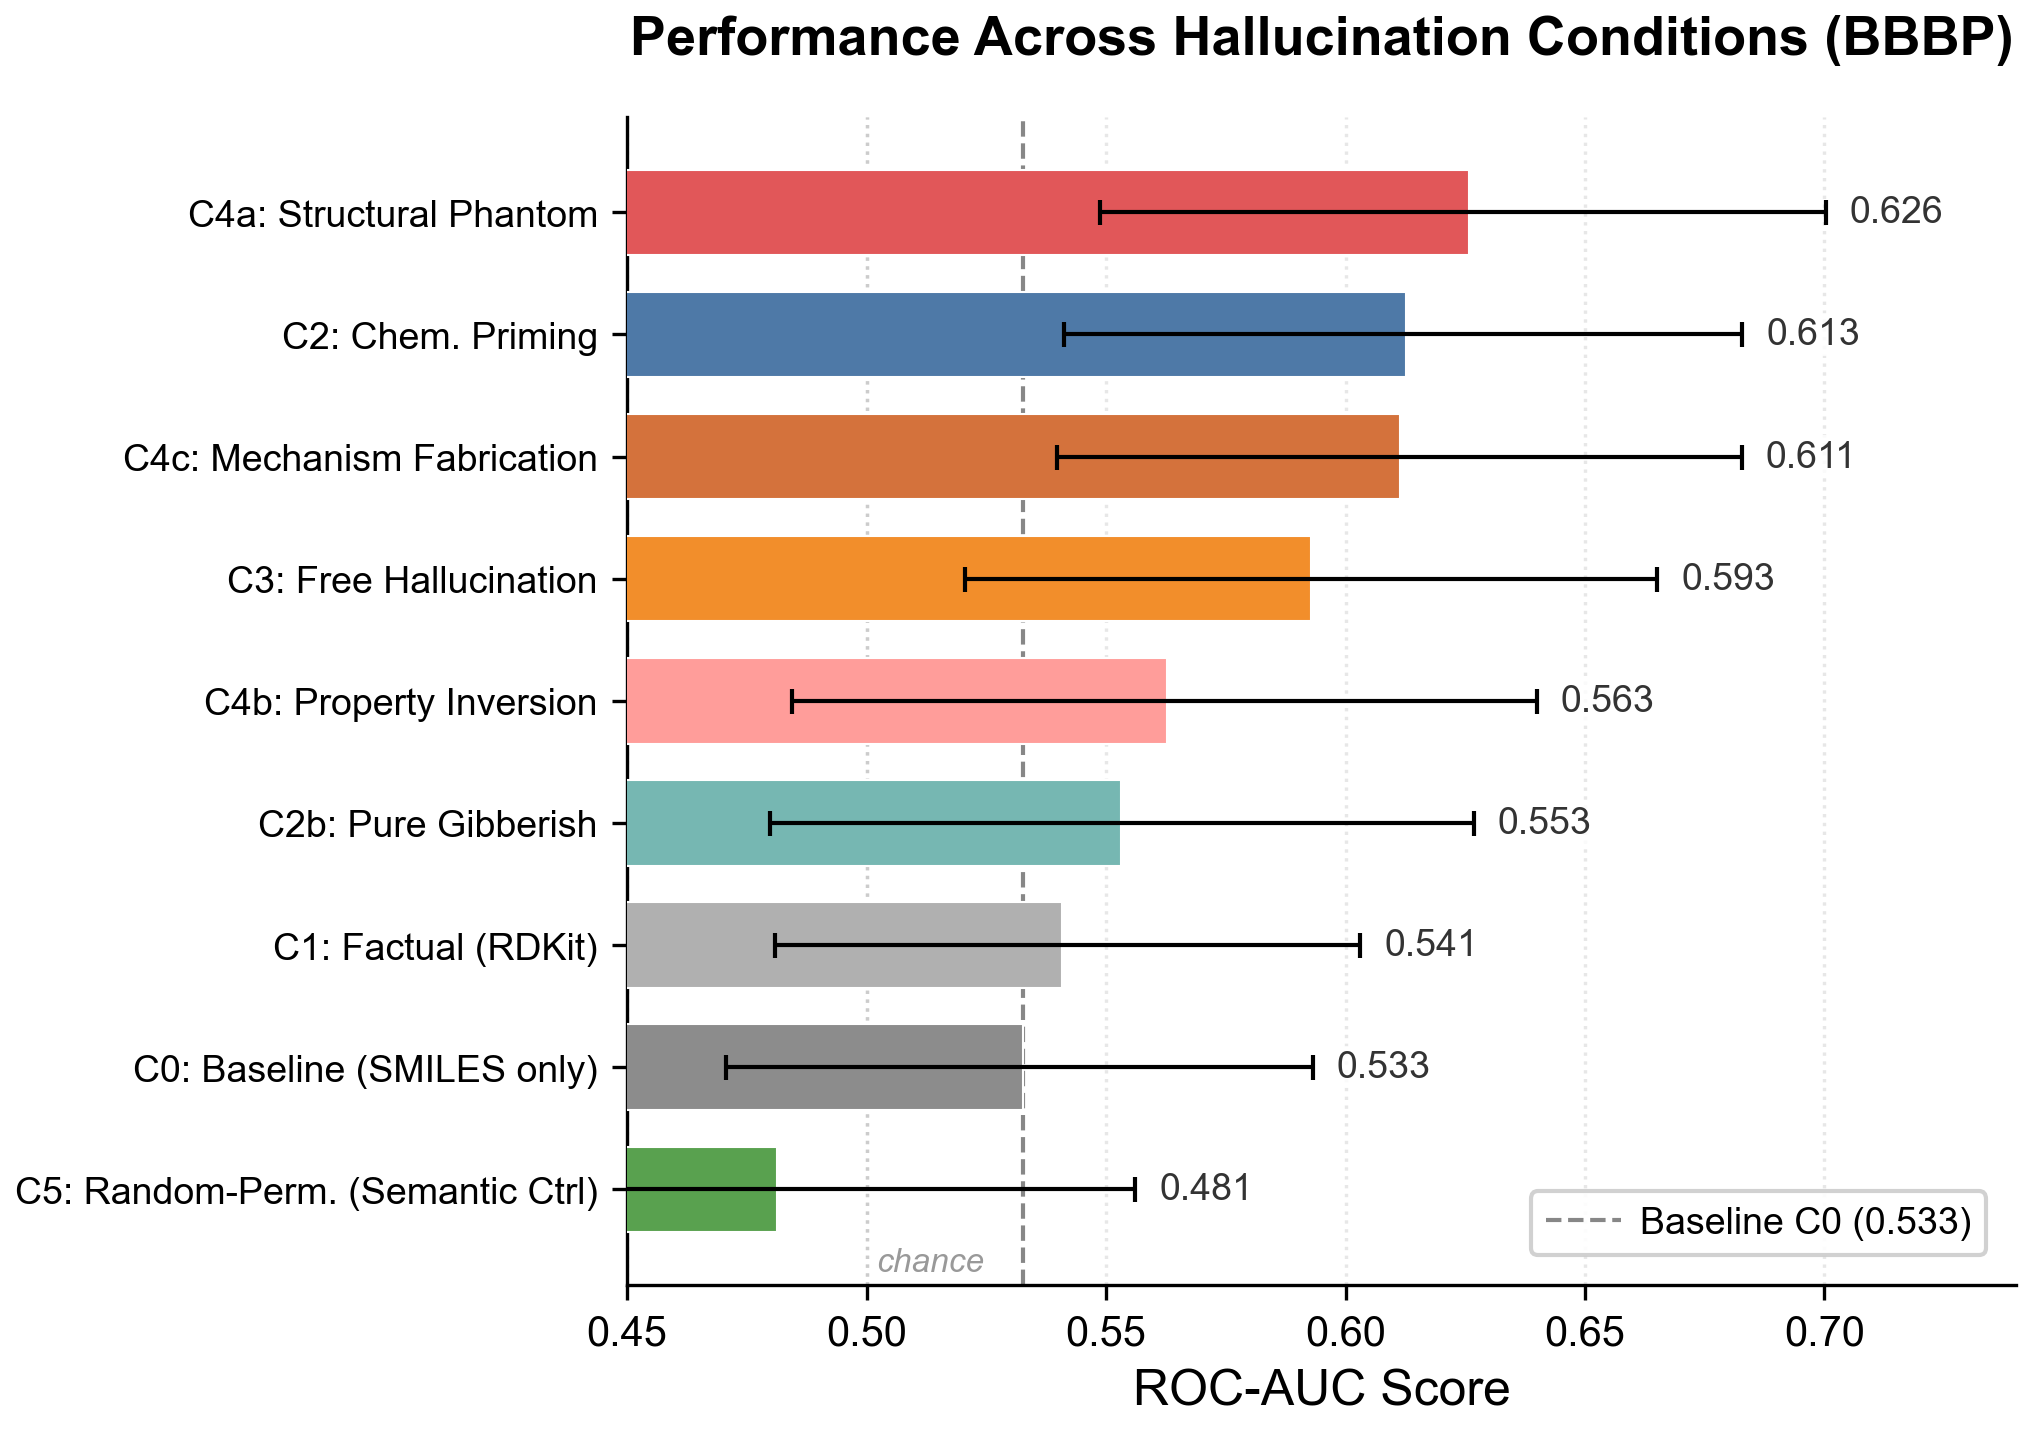
\includegraphics[width=\linewidth]{figures/figure1_performance_comparison.png}
    \caption{Task-dependent divergence in hallucination sensitivity across perturbation conditions, with structurally grounded (SP) hallucination associated with the largest discriminative improvement on BBBP.}
    \label{fig:performance}
\end{figure}

\subsubsection{BBBP (Physicochemical Task)}
To contextualize the LLM zero-shot performance, the traditional ML baseline (Random Forest with Morgan fingerprints) achieved an expectedly strong ROC-AUC of 0.705 on the BBBP test set. While the zero-shot LLM predictions remain strictly below this traditional baseline, the relative differences between textual augmentation conditions reveal substantial semantic perturbation effects.

The LLM baseline (C0, SMILES only) yielded a ROC-AUC of 0.533 [0.471, 0.593]. Factual augmentation (C1) produced a marginal, non-significant increase to 0.540. Chemical priming (C2) yielded 0.614, while pure non-chemical gibberish (C2b) yielded 0.553.

Free hallucination (C3) improved ROC-AUC to 0.594 [0.519, 0.664]. Among category-specific conditions, Structural Phantom hallucination (C4a) yielded the highest observed ROC-AUC of 0.626 [0.548, 0.698], followed by Mechanism Fabrication (C4c, 0.612) and Property Inversion (C4b, 0.561). 

\paragraph{Bootstrap Stability.} To account for the single-split evaluation, we computed ranking stability across 1,000 bootstrap resamples (Figure~\ref{fig:bootstrap}). The superiority of SP hallucination (C4a) over the LLM baseline (C0) proved highly stable, maintaining a positive margin in 97.6\% of resamples. Free hallucination (C3) outperformed the baseline in 87.7\% of resamples.

\begin{figure}[h]
    \centering
    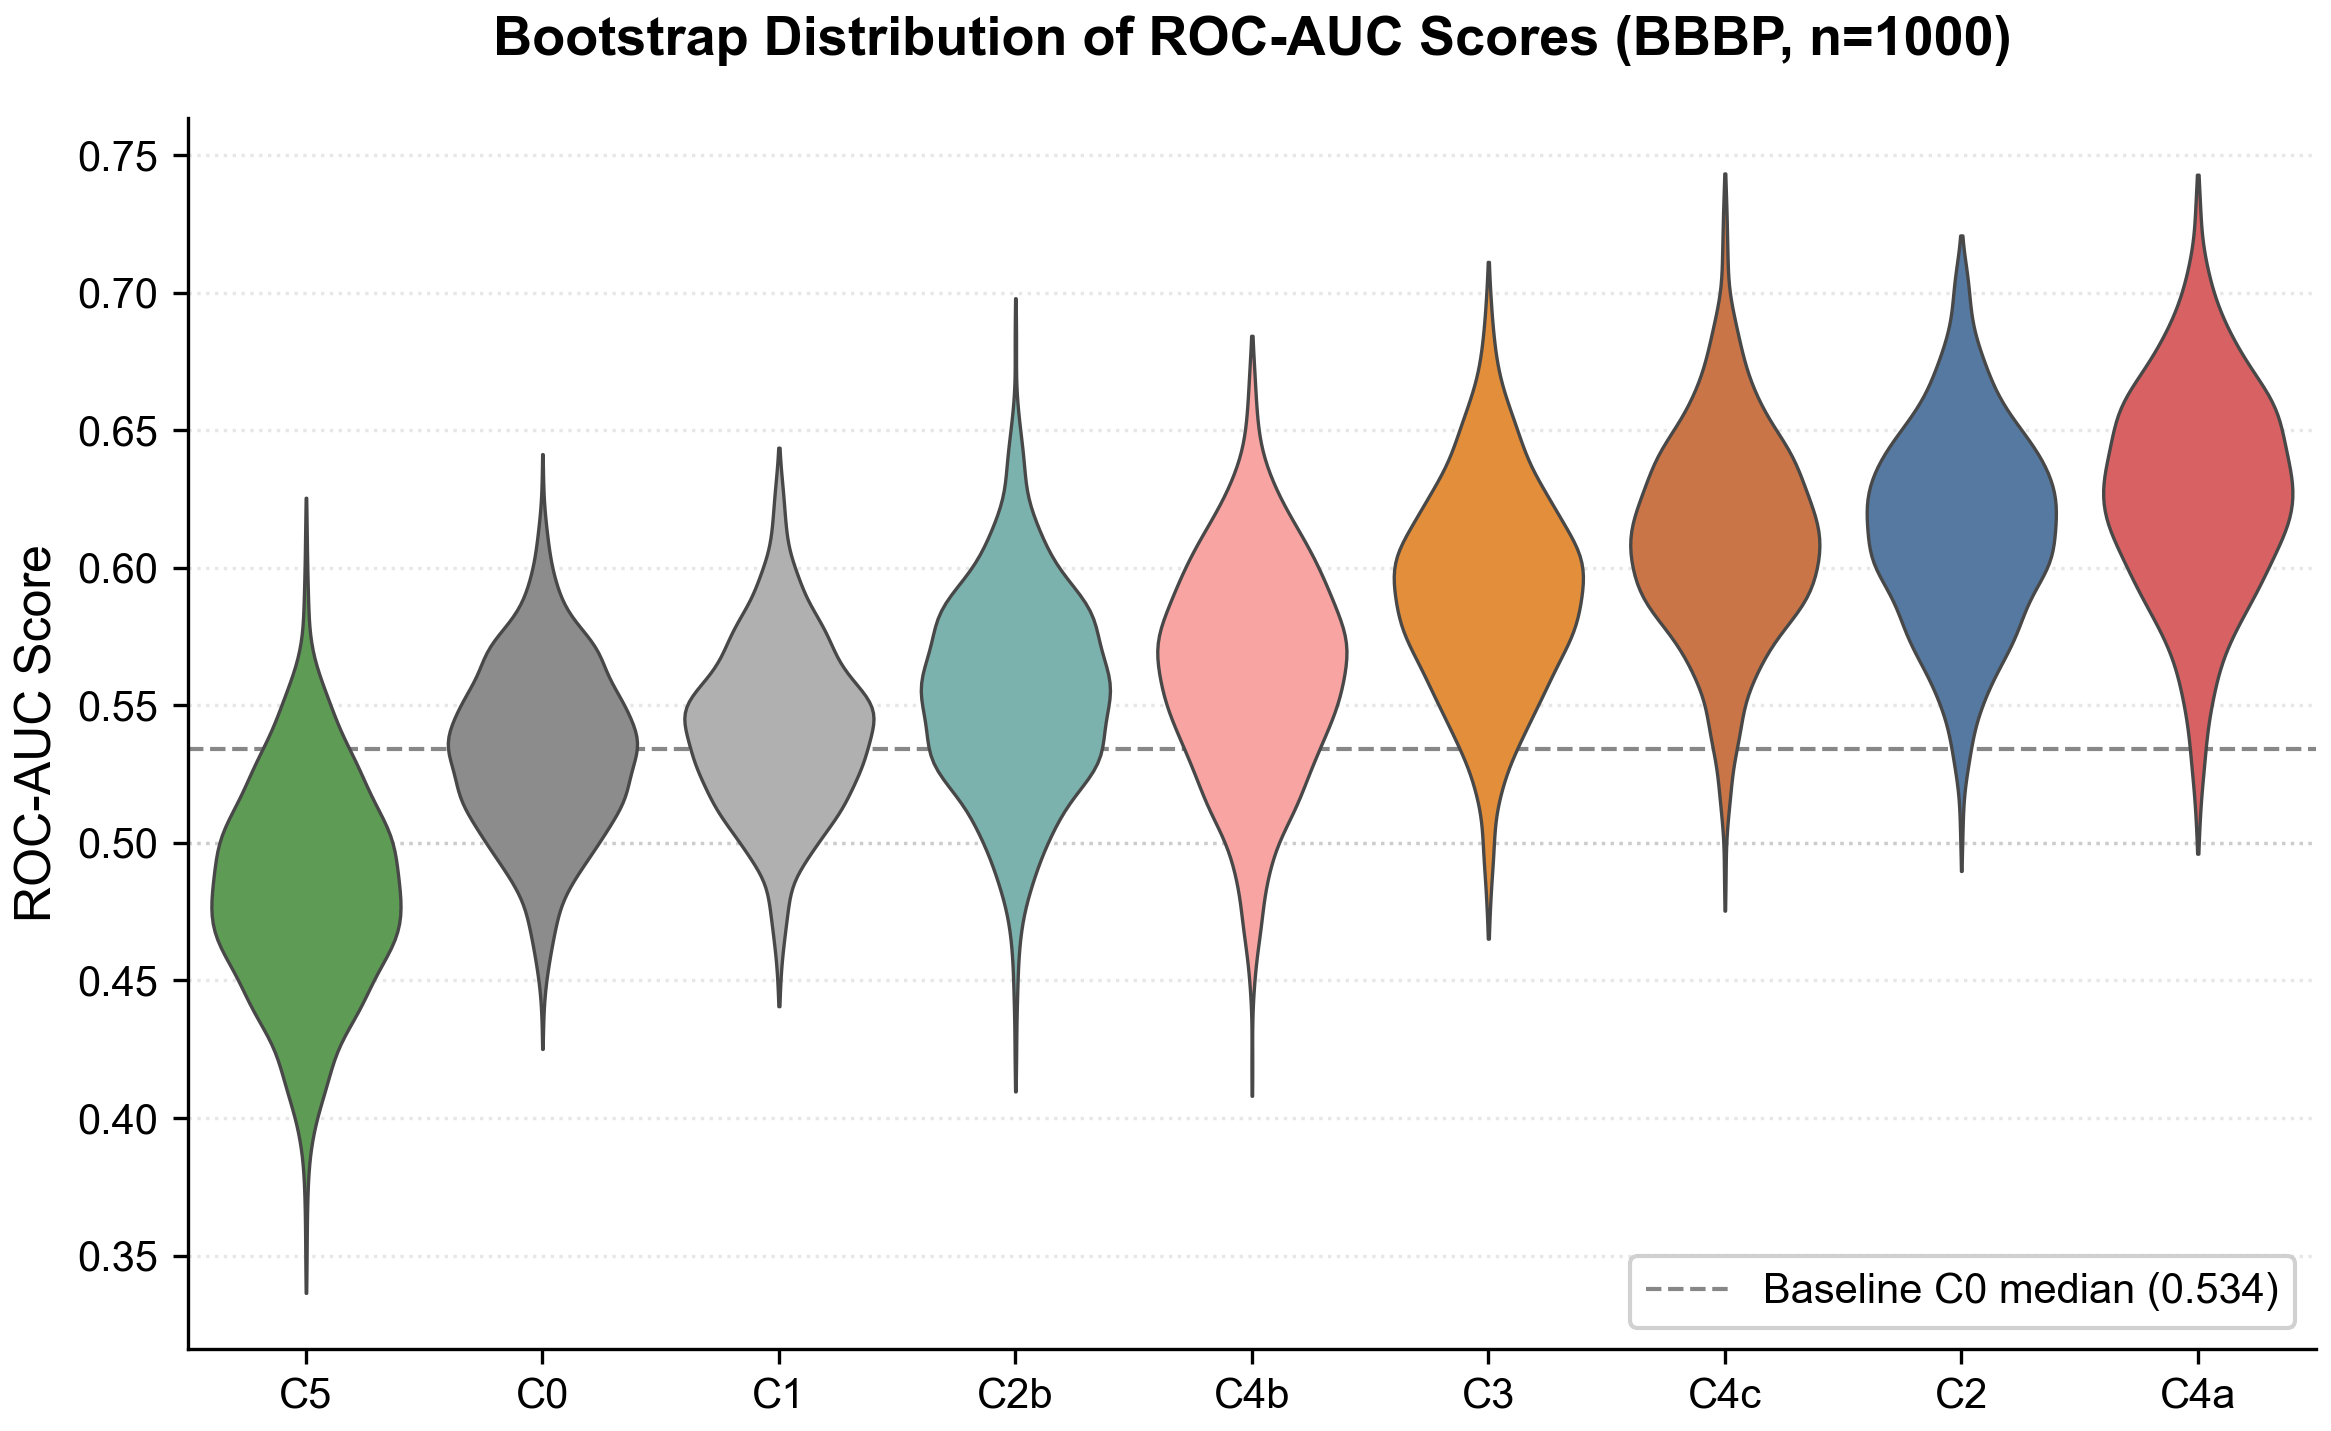
\includegraphics[width=0.8\linewidth]{figures/figure2_bootstrap_stability.png}
    \caption{Bootstrapped ROC-AUC distributions demonstrate the statistical stability of Structural Phantom (C4a) hallucination gains relative to the SMILES baseline (C0) on the BBBP dataset.}
    \label{fig:bootstrap}
\end{figure}

The circular-shift semantic control (C5) yielded 0.530 [0.454, 0.607], closely aligned with baseline C0 and substantially below C3, indicating that the scientific register of hallucinated text alone does not account for the observed gains.

\subsubsection{BACE (Enzymatic Task)}
On the BACE test set ($N=152$), a contrasting pattern was observed. The baseline (C0) yielded a ROC-AUC of 0.656 [0.556, 0.752]. All hallucination-augmented conditions reduced performance relative to baseline. Free hallucination (C3) reduced ROC-AUC to 0.488 [0.389, 0.589], representing a substantial degradation toward near-chance behavior.

\subsection{Prediction Collapse on BACE}
Under hallucination conditions on BACE, the distribution of predicted probabilities collapsed from a bimodal pattern (reflecting the model's baseline discriminative behavior) to a narrow unimodal distribution centered at $p \approx 0.17$, regardless of the molecule's true label. This effect, which we descriptively term ``prediction collapse,'' was observed across all hallucination conditions (C3, C4a--c) and suggests systematic signal destruction rather than random noise injection.

\begin{figure}[t]
    \centering
    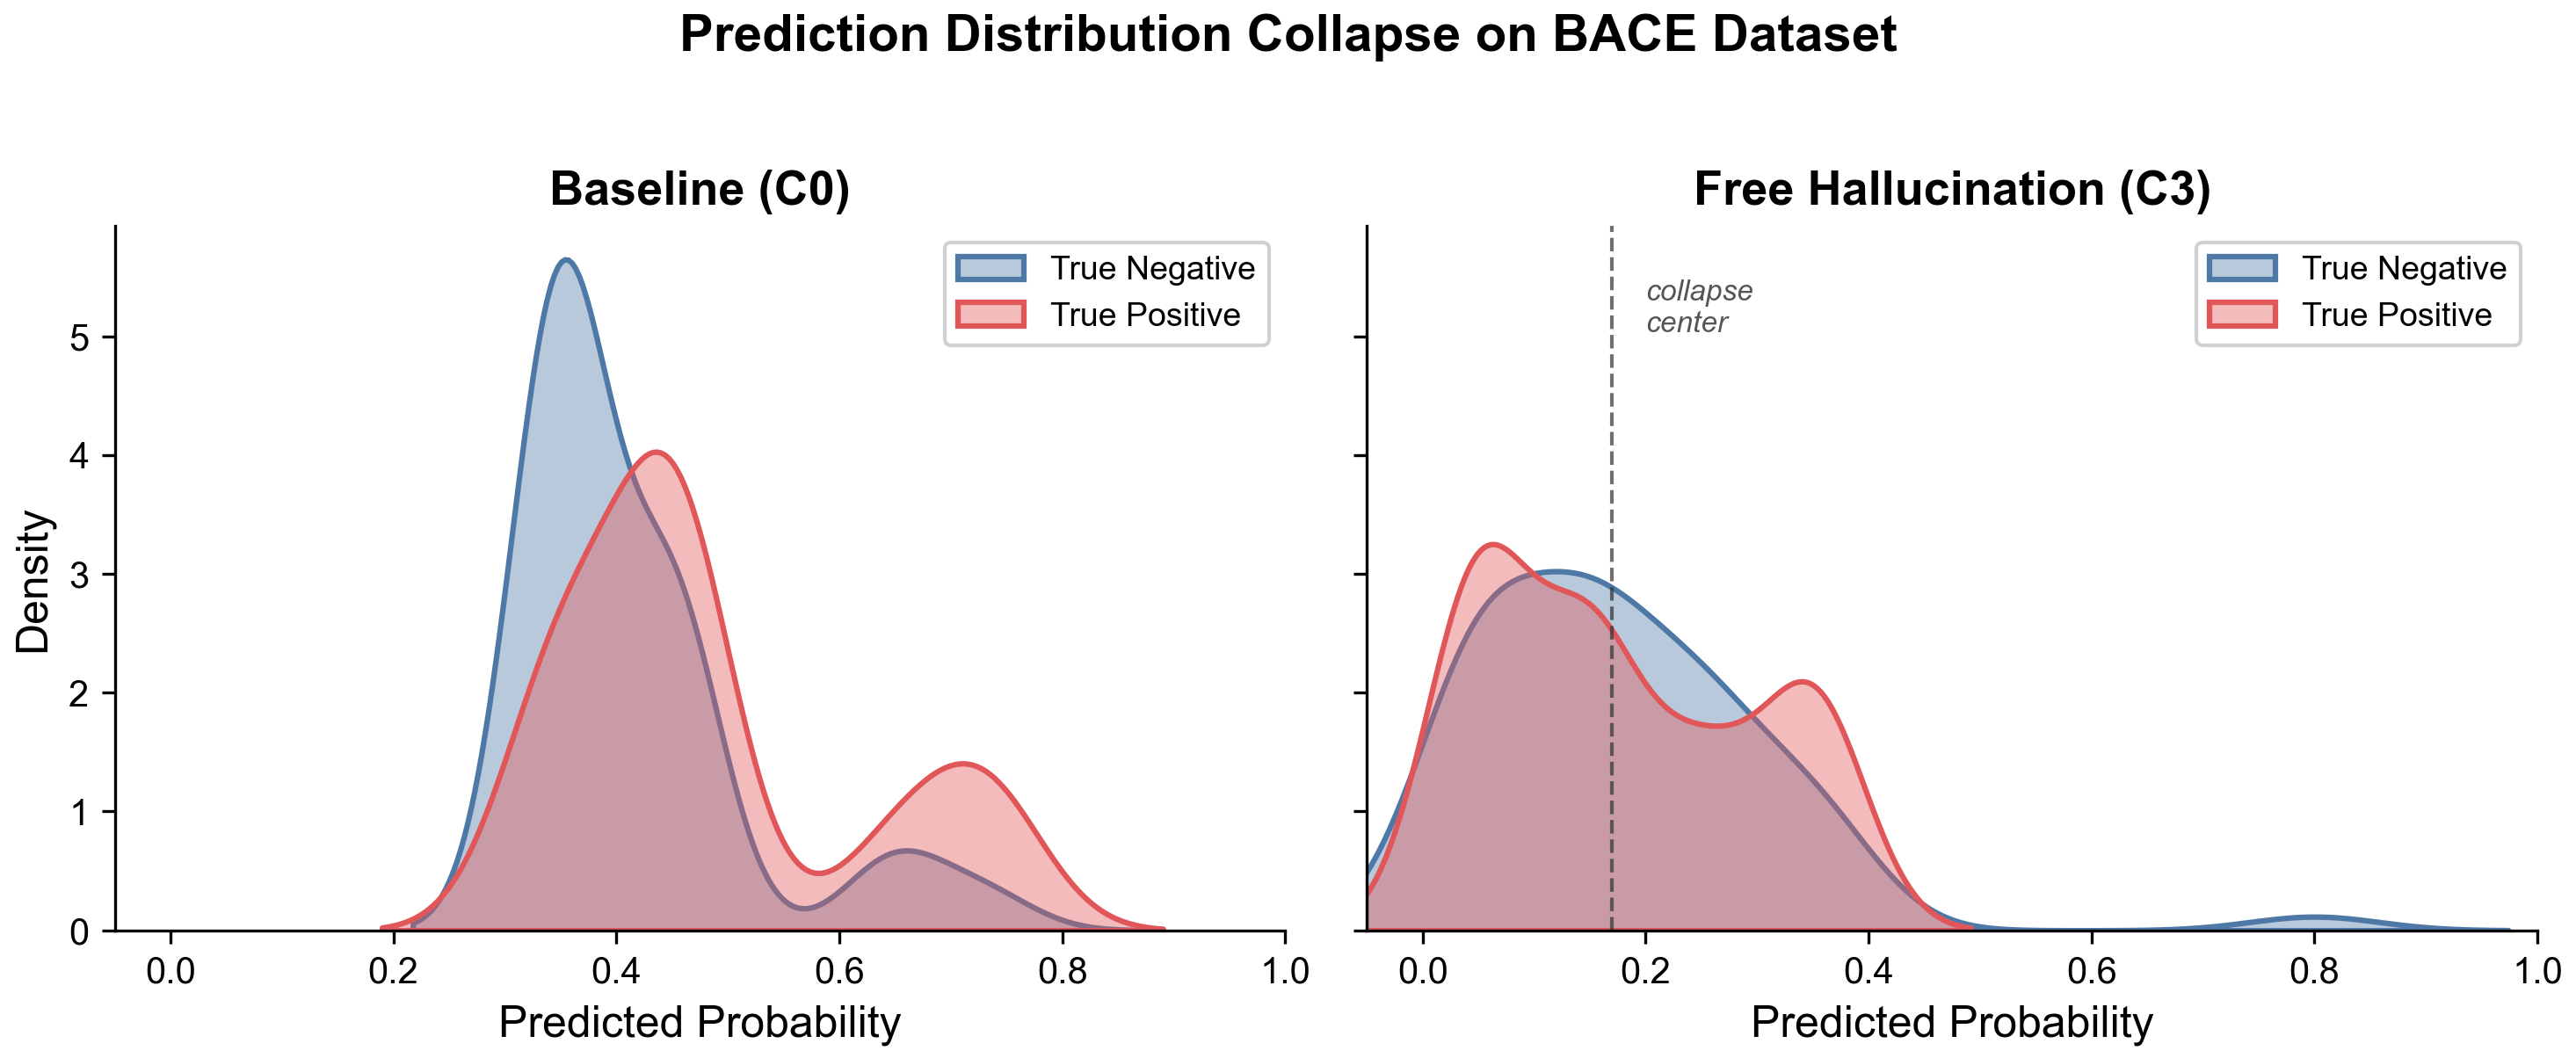
\includegraphics[width=\linewidth]{figures/figure3_negativity_collapse.png}
    \caption{Hallucination augmentation induces pronounced distributional compression on the BACE task, shifting the baseline bimodal prediction distribution toward a non-discriminative narrow peak near $p \approx 0.17$.}
    \label{fig:negativity}
\end{figure}

\subsection{Distribution of Hallucination Types}
Analysis of 356 naturally generated hallucinations across both datasets revealed a consistent distributional bias (Figure~\ref{fig:taxonomy}). Contextual Confabulation (CC) was the dominant category, accounting for approximately 80\% of all generated descriptions ($n=163$ of 204 for BBBP). Structural Phantom (SP) was the rarest category at 2.4\% ($n=5$ of 204 for BBBP). Despite this low natural frequency, forced SP hallucinations (C4a) exhibited the strongest predictive association on BBBP.

\begin{figure}[t]
    \centering
    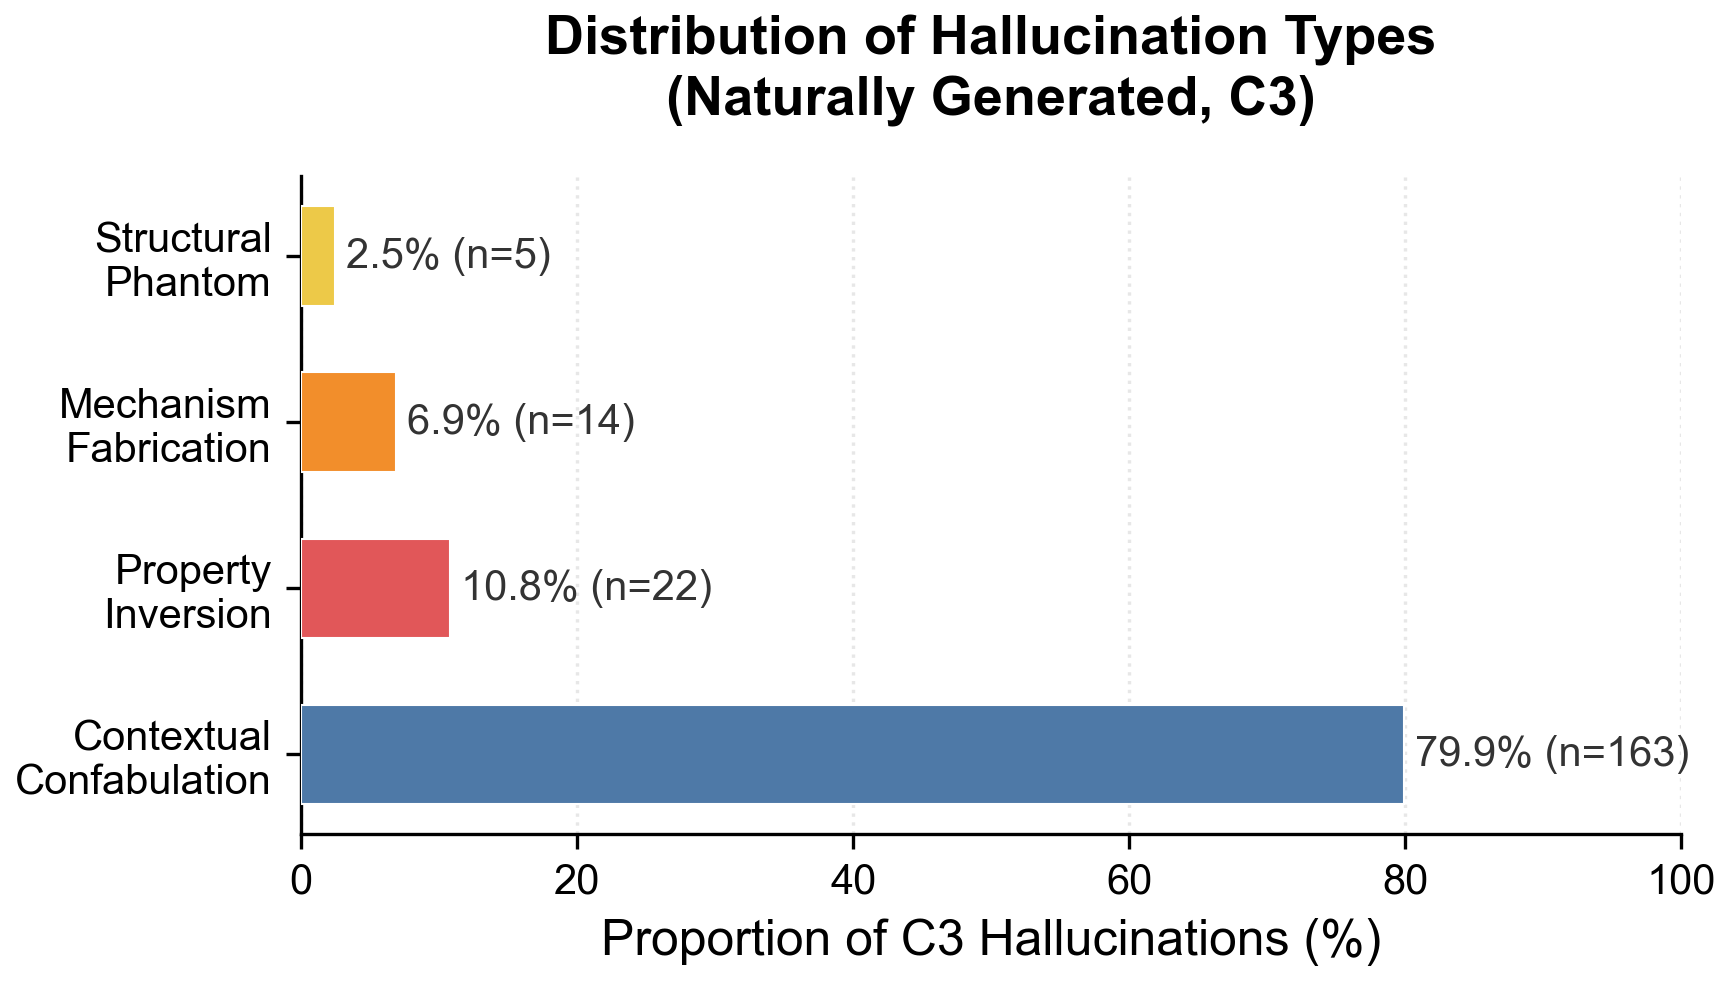
\includegraphics[width=0.8\linewidth]{figures/figure4_taxonomy_distribution.png}
    \caption{Free hallucinations exhibit a pronounced distributional bias toward generic Contextual Confabulation (CC), with structurally grounded perturbations (SP) occurring rarely despite their stronger association with predictive performance.}
    \label{fig:taxonomy}
\end{figure}

\section{Discussion}

The results of this study suggest that LLM-based molecular 
property prediction exhibits systematic sensitivity to structured 
semantic perturbations, with the direction and magnitude of 
observed effects depending on the task domain.

\subsection{Textual Augmentation as Semantic Conditioning}
A primary finding of this study is that the \textit{semantic 
orientation} induced by a prompt---the topical focus on specific 
molecular features---is a consistent driver of predictive 
shifts, often more so than the factual taxonomic correctness of the generated 
text. This was observed in the C4a (Structural) condition, 
where the LLM generated contextually plausible descriptions 
focused on structural features but failed to satisfy the strict 
Structural Phantom definition (i.e., referencing absent 
elements). Despite this taxonomic non-compliance, C4a 
consistently yielded the largest directional ROC-AUC 
improvements on BBBP and Tox21 while preserving baseline 
discriminability on BACE and yielding a marginal directional improvement over C0 on ESOL (RMSE: 2.045 vs.\ 2.051).

We frame this pattern as an effect of \textit{semantic conditioning}: the 
observation that factually non-compliant but topically 
structured text can systematically shift prediction behavior 
in a task-dependent direction. We emphasize that this 
characterization is descriptive and behavioral---it refers to 
the observed co-occurrence of structural topic focus and 
directional performance shifts, and does not constitute a 
mechanistic claim about the model's internal processing.

\subsection{Distributional Compression on Enzymatic and 
Solubility Tasks}
The consistent performance degradation observed on BACE and ESOL provides evidence that textual augmentation is systematically harmful in specific task regimes, though the effect is modulated by both vocabulary and molecular specificity. Notably, the enzymatic regime appears particularly sensitive to chemical-domain vocabulary presented in a generic, non-molecule-specific context---as evidenced by the significant degradation in C2 ($p_{\text{BH}}=0.011$) and factual C1 ($p_{\text{BH}}=0.011$). Conversely, pure non-chemical gibberish (C2b, $p_{\text{BH}}=0.217$) and molecule-specific structural descriptions (C4a, $p_{\text{BH}}=0.808$) did not induce statistically significant performance loss. This pattern suggests that the disruptive mechanism on enzymatic tasks is primarily driven by domain-relevant but generic contextual noise that displaces the SMILES representation, while specific structural anchoring (C4a) or completely irrelevant register (C2b) is less disruptive. This indicates that while fabrication leads to entropy collapse, distributional noise from generic chemical-rich text is equally disruptive to prediction ranking.

Quantitatively, this is reflected in the calibration metrics 
reported in Table~\ref{tab:calibration}. Under the C3 
condition on BACE, Brier Score increased from 0.244 to 0.438 
and ECE from 0.151 to 0.439---indicating that hallucination 
augmentation does not merely introduce ranking noise, but 
systematically degrades probability calibration. This 
behavioral pattern, which we term \textit{distributional 
compression}, consists of a collapse of the model's output 
distribution toward a narrow low-confidence peak near 
$p \approx 0.17$, regardless of true label. This is distinct 
from regression toward the BACE test set's class prior 
(60.5\% positive), indicating a genuine loss of 
discriminative signal rather than label-frequency anchoring.

One plausible account is that fabricated enzymatic or solubility claims introduce conflicting contextual signals that override the limited structural information conveyed by the SMILES input, collapsing the model's output toward a non-discriminative state. However, we note that this account remains speculative in the absence of mechanistic interpretability analysis. Crucially, the enzymatic regime is sensitive to any textual augmentation that shifts the model's attention away from SMILES-derived features. A notable exception is the prompt-constrained structural condition (C4a), which preserved baseline AUC (0.666 vs.\ 0.674) and substantially improved calibration (ECE: 0.069 vs.\ 0.151). This asymmetry suggests that the structural topic focus of C4a may anchor the model's attention to features that are complementary to SMILES parsing, whereas generic descriptor strings or fabricated claims introduce distributional noise that overwhelms the model's limited enzymatic reasoning capacity.

\subsection{Scaling Divergence and Representational States}
A critical observation in our scaling exploration (Section~\ref{sec:implementation_robustness}) is the divergence in behavior between Llama-3.1-8B and Llama-3.3-70B on the BBBP task. While the 8B model exhibited directional improvements with structural augmentation, the 70B model showed directional degradation when evaluated on the same textual augmentations. This reversal suggests that the ``utility'' of semantic augmentation is not an intrinsic property of the text itself, but is a function of the model's baseline representational state. If a larger model already captures the necessary structural information from the SMILES input, the addition of textual descriptions (especially those generated by a smaller 8B model) may introduce harmful interference rather than helpful conditioning. This underscores the necessity of task-specific and model-specific calibration when deploying text-augmented molecular reasoning systems.

\subsection{Generalization and Pre-training Artifacts}
The contrast between BBBP/Tox21 and BACE/ESOL suggests that 
task sensitivity may correlate with the prevalence of 
structural reasoning vs.\ specific mechanistic retrieval 
in the pre-training distribution. General physicochemical 
properties---such as blood-brain barrier permeability and 
broad toxicity---are more broadly represented in the 
scientific literature in association with diverse molecular 
scaffolds. In these domains, structural topic focus (C4a) 
may prime the model's contextual inference toward relevant 
sub-graph patterns, producing directional ROC-AUC 
improvements even without factual accuracy. Specific enzymatic mechanisms and 
quantitative solubility, by contrast, may be less densely 
covered in general-domain pre-training corpora, making 
predictions in these regimes more susceptible to disruption 
by fabricated claims.

We note that this interpretation is speculative and cannot 
be verified without targeted analysis of training data 
composition or model internals, which is beyond the scope 
of this exploratory study.

The observed cross-task consistency also suggests that 
semantic perturbation experiments of this kind may serve 
as a lightweight behavioral probe for characterizing 
task-specific inference sensitivity in LLMs---one that 
does not require access to model weights or internal 
representations, and can be applied to black-box API-based 
systems. We make no stronger claim about the mechanistic 
basis of this sensitivity.

\subsection{Methodological Implications}
Our findings carry several practical implications for 
LLM-augmented cheminformatics. First, the observed 
directional trend of structural topic-focus prompting (C4a) over 
factual RDKit descriptors (C1) on physicochemical tasks 
suggests that topically oriented textual context may 
sometimes provide a more effective inference substrate for 
general-purpose LLMs than numerical descriptor strings, 
which may not integrate naturally into language-based 
reasoning chains. Second, the severe calibration failure 
on BACE---reflected in ECE values approaching 0.44---
underscores the risk of deploying LLM-augmented 
predictions in enzymatic domains without explicit 
uncertainty quantification. Future work should examine 
whether calibration-aware prompting strategies or 
post-hoc recalibration can mitigate this effect.

\section{Limitations}
\label{sec:limitations}

This study has several important limitations that constrain the generalizability and interpretability of its findings.

\subsubsection*{Model scope.} Primary experiments were conducted with Llama-3.1-8B-Instant. While cross-model validation was performed with Llama-3.3-70B, this was limited to two conditions (C0, C3) and a single inference run, precluding a full nine-condition multi-seed ablation for the larger architecture. The observed effects—including the task-dependent performance asymmetry—may be sensitive to model family, parameter count, or inference backend beyond the two evaluated scales.

\subsubsection*{Single-split evaluation.} Results are based on a single scaffold-split test set for each dataset (BBBP $N=204$, BACE $N=152$) without full cross-validation. This makes the reported ROC-AUC values sensitive to the specific test partition. While we employed multi-seed resampling to evaluate generative stability (Table~\ref{tab:robustness}), extending this framework to multiple independent scaffold splits is required to definitively isolate generalizable phenomena from dataset-specific artifacts. We explicitly defer this multi-split validation to future work, positioning the current findings as exploratory behavioral probes rather than comprehensive benchmarks.

\subsubsection*{Limited sample size.} With 204 and 152 molecules respectively, this study is underpowered for detecting small but potentially meaningful effect size differences between conditions. The SP category comprised only 5 naturally occurring instances in BBBP, making any distributional claims about SP highly tentative.

\subsubsection*{C2 control confound.} The chemical priming condition (C2) contains domain-relevant vocabulary (``structural'', ``molecular'', ``physicochemical''), making it a partial rather than pure stylistic control. While C2b addresses this with non-chemical vocabulary, the C2 results should be interpreted with this confound in mind.

\subsubsection*{Taxonomy and Classifier Validity.} The heuristic classification scheme used to categorize free hallucinations (C3) into SP, PI, MF, or CC is an unvalidated rule-based system. To assess its reliability, we conducted an AI-assisted semantic validation on a stratified sample ($N=70$) using an LLM-as-judge approach (Llama-3.1-8B-Instant). The agreement between the heuristic classifier and the semantic judge was poor (Cohen's $\kappa = 0.117$, raw agreement 44.3\%), with the LLM judge exhibiting severe overclassification toward Mechanism Fabrication (MF) and failing to reliably identify Structural Phantoms (SP) or Property Inversions (PI). This high disagreement rate highlights the inherent ambiguity in categorizing generative chemical text. Consequently, the categories (SP, PI, MF, CC) should be interpreted strictly as \textit{prompt design intents} or heuristic keyword clusters, rather than definitive semantic truths. The Contextual Confabulation (CC) category functions as a catch-all residual class, encompassing heterogeneous subtypes whose homogeneous treatment obscures important variations. This limitation is further evidenced by the post-hoc verification of C4a--c outputs (Table~\ref{tab:c4_compliance}): despite prompt-constrained forcing, C4a achieved 0\% target compliance (SP), C4b achieved 25.5\% (PI), and C4c achieved 20.4\% (MF), with CC dominating all three conditions ($\geq$74\%). This systematic prompt--output misalignment demonstrates the challenge of enforcing strict semantic perturbation categories in generative chemistry pipelines.


\subsubsection*{Data leakage risk.} As highlighted in recent literature~\cite{guo2023benchmark, white2023assessment}, modern LLM pre-training corpora (such as those used for Llama and Gemma) likely encompass massive amounts of public chemical data, including the MoleculeNet datasets. Consequently, the zero-shot predictions evaluated here may partially reflect varying degrees of memorized retrieval rather than pure inferential reasoning. While our control conditions (C5) demonstrate that structural prompts without semantic alignment fail to produce predictive gains, hallucinated text might inadvertently trigger memorized associations, collapsing the evaluation framework from a test of reasoning to a test of prompted recall.

\subsubsection*{API non-determinism.} Despite setting temperature $= 0.0$ and seed $= 42$, Groq's API documentation notes that seed-based reproducibility is provided on a best-effort basis. Exact numerical reproducibility across runs is therefore not guaranteed.

\subsubsection*{ESOL Task Framing.} Our ESOL evaluation used a zero-shot regression prompt. However, as LLMs are typically optimized for categorical text output rather than high-precision scalar regression, the reported RMSE reflects the inherent limitations of zero-shot regression in the absence of specialized prompting or fine-tuning. These values should be interpreted as a relative measure of semantic sensitivity across augmentation conditions rather than an absolute measure of solubility prediction accuracy.

\subsubsection*{Dataset scope.}
The primary nine-condition ablation was conducted on two 
MoleculeNet benchmarks (BBBP and BACE), with targeted 
three-condition generalization validation on Tox21 and 
ESOL. Full nine-condition ablation on Tox21 and ESOL, 
and extension to additional task types such as protein 
binding affinity, remains reserved for future work. 
Cross-dataset generalization of the observed 
distributional compression phenomenon should be 
interpreted with caution given the limited condition 
coverage of the extended benchmarks.

\subsubsection*{Inference-only evaluation.} While we include a traditional ML baseline (Random Forest) for context, we evaluate only zero-shot LLM inference. Comparison with fine-tuned LLM models would provide additional context for the practical significance of the observed effects.

\subsubsection*{Methodological confounds.} The BACE Mechanism Fabrication (C4c) condition directly prompts the LLM to hypothesize biological targets. Because BACE-1 is the implied target of the BACE dataset, the MF text may inadvertently contain information about BACE-1 itself, creating a direct semantic confound rather than a general structural perturbation. Although we validated the C5 control across multiple permutation seeds ($0.49 \pm 0.02$), a larger number of permutations with full-dataset evaluation would further strengthen this control.

\section{Conclusion}
\label{sec:conclusion}

In this work, we introduced a controlled semantic perturbation framework to evaluate how structured hallucinations influence LLM-based molecular property prediction. Our results reveal a task-dependent divergence in semantic sensitivity: physicochemical prediction (BBBP) exhibits directional sensitivity to structural topic focus, while enzymatic reasoning (BACE) is robustly fragile to semantic fabrication. Crucially, we find that the semantic orientation induced by a prompt can drive predictive shifts even in the absence of factual taxonomic correctness, suggesting that hallucinations may act as a form of semantic regularization that activates latent chemical priors. 

These findings indicate that structured hallucinations are not merely errors, but informative perturbations that can be leveraged to probe the latent reasoning dynamics of LLMs. This study provides a structured methodological foundation for future work investigating the boundary between linguistic register and semantic utility in text-conditioned molecular prediction pipelines.

\subsubsection*{Future directions.} Key extensions include: (1) investigation of the distributional compression phenomenon on additional enzymatic datasets, (2) expansion of multi-model validation across diverse LLM architectures and scales, (3) larger-scale evaluation with cross-validation, and (4) comparison with fine-tuned LLM models and additional traditional ML methods to further contextualize the practical significance of the observed effects.


\section*{CRediT authorship contribution statement}
\textbf{Muhammad Afif Erdita:} Conceptualization, Data Curation, Formal Analysis, Investigation, Methodology, Project Administration, Software, Validation, Visualization, Writing -- Original Draft, Writing -- Review \& Editing.

\section*{Declaration of competing interests}
The author declares that there are no known competing financial interests or personal relationships that could have appeared to influence the work reported in this paper.

\section*{Data availability}
The complete codebase, generated datasets, and high-resolution figures are publicly available at: \url{https://github.com/apiprdt/AI-Hallucinations}. A static version of the evaluation datasets is provided within the repository to ensure exact reproducibility.

\section*{Acknowledgments}
The author acknowledges the use of \texttt{Llama-\allowbreak 3.1-\allowbreak 8B-\allowbreak Instant} and \texttt{Llama-\allowbreak 3.3-\allowbreak 70B-\allowbreak Versatile} (via Groq API) for hallucination generation and molecular prediction inference. Large language models were also used for assistance in drafting and revising sections of this manuscript.

\bibliographystyle{elsarticle-num}
\bibliography{references}

\newpage
\appendix
\section{Appendix}
\label{sec:appendix}

\subsection{Prediction Prompt Templates}
All prediction queries used temperature $= 0.0$, \texttt{max\_tokens} $= 10$, and seed $= 42$. The augmentation line is omitted for C0.

\subsubsection*{Primary Ablation (BBBP, BACE):}
\begin{verbatim}
Given this molecule (SMILES: {smiles})
[Additional information: {augmentation}]

On a scale of 0 to 1, what is the probability
that this molecule can {task_description}?
Respond with ONLY a number between 0 and 1.
Nothing else.
\end{verbatim}
Task descriptions: ``penetrate the blood-brain barrier'' (BBBP), ``inhibit the BACE-1 enzyme'' (BACE).

\subsubsection*{Extended Benchmark: Tox21 (Classification):}
\begin{verbatim}
Given this molecule (SMILES: {smiles})
[Additional information: {augmentation}]

Is this molecule toxic for the NR-AR pathway?
Respond with ONLY a number representing the
probability of toxicity (between 0 and 1).
Nothing else.
\end{verbatim}

\subsubsection*{Extended Benchmark: ESOL (Regression):}
\begin{verbatim}
Given this molecule (SMILES: {smiles})
[Additional information: {augmentation}]

What is the measured log solubility in mols
per litre for this molecule?
Respond with ONLY a numerical value (e.g.,
-2.5). Nothing else.
\end{verbatim}

Hallucination generation used temperature $= 0.9$, \texttt{max\_tokens} $= 150$, with the following type-specific prompts.

\subsubsection*{Primary Ablation Generation Prompts (BBBP, BACE):}

\textbf{C3 (Free Hallucination):}
\textit{``You are a speculative chemist. Given SMILES: \{smiles\}. Generate a creative, scientifically-sounding description of this molecule's potential properties and biological mechanisms. Be creative and speculative. Write 2--3 sentences only.''}

\textbf{C4a (Structural Augmentation):}
\textit{``Given SMILES: \{smiles\}. Describe the structural features, functional groups, and atomic composition. Be specific and speculative.''}

\textbf{C4b (Property Inversion):}
\textit{``Given SMILES: \{smiles\}. Describe its solubility, lipophilicity, and membrane permeability with specific values.''}

\textbf{C4c (Mechanism Fabrication):}
\textit{``Given SMILES: \{smiles\}. Hypothesize biological targets and cellular mechanisms. Be specific about protein targets.''}

\subsubsection*{Extended Benchmark Generation Prompts (Tox21, ESOL):}
\textbf{Note:} The generation prompts for the extended benchmarks were adapted from the primary ablation prompts. While designed to serve the same functional role, the exact phrasing differs, which constitutes a minor methodological confound acknowledged in the main text.

\textbf{C3 (Free Hallucination):}
\textit{``Provide a detailed scientific description of the molecular structure and properties for the molecule with SMILES: \{smiles\}. Focus on its potential biological interactions and physicochemical characteristics.''}

\textbf{C4a (Structural Augmentation):}
\textit{``Describe the scaffold and structural features of the molecule with SMILES: \{smiles\}. Mention specific rings, functional groups, and their spatial arrangement.''}

\subsection{Control Condition Templates}

\subsubsection*{C2 (Chemical Priming):}
Template-generated text using scientific vocabulary:
\textit{``This compound exhibits \{adj\} structural coherence with \{noun\} interaction domains, demonstrating \{adj\} physicochemical characteristics under \{noun\} conditions.''}

Adjective pool: moderate, intermediate, variable, standard, conventional, typical.
Noun pool: hypothetical, theoretical, computational, structural, molecular, chemical.

\textbf{Note:} This template contains chemical vocabulary (``structural'', ``molecular'', ``physicochemical''), making C2 a \emph{partial} stylistic control. See C2b for the stricter control.

\subsubsection*{C2b (Pure Gibberish):}
Template-generated text using exclusively non-chemical vocabulary:
\textit{``This entity exhibits \{adj\} portfolio coherence with \{noun\} governance domains, demonstrating \{adj\} bureaucratic characteristics under \{noun\} conditions.''}

Adjective pool: variable, standard, conventional, typical, moderate, intermediate.
Noun pool: portfolio, transactional, governance, bureaucratic, administrative, regulatory.

Vocabulary audit confirmed 0\% overlap with a curated chemical/biological term list.

\subsection{Taxonomy Classifier Pseudocode}

\begin{enumerate}
    \item \textbf{SP Detection:} For each element in \{F, Cl, Br, I, P, S, N\}, check if associated keywords appear in the generated text. Cross-reference with \texttt{mol.GetAtoms()} to verify element absence. If a keyword matches an absent element, classify as SP.
    \item \textbf{PI Detection:} Compute MolLogP via RDKit. If LogP $> 3$ and text contains ``water soluble'', ``hydrophilic'', or ``highly soluble'', classify as PI. If LogP $< 1$ and text contains ``lipophilic'', ``hydrophobic'', or ``membrane permeable'', classify as PI.
    \item \textbf{MF Detection:} Keyword matching for 9 biological targets: ACE2, HER2, EGFR, VEGF, p53, BCL-2, COX-2, dopamine, serotonin.
    \item \textbf{CC (Default):} If none of the above conditions trigger, classify as Contextual Confabulation.
\end{enumerate}

\subsection{Representative Hallucination Examples}
\begin{itemize}
    \item \textbf{SP Example (SMILES: c1ccccc1, Benzene):} ``Contains a reactive chlorine atom that enhances metabolic stability.'' (Benzene contains no chlorine atoms.)
    \item \textbf{PI Example (SMILES: high-LogP compound):} ``This highly water-soluble molecule readily dissolves in aqueous media.'' (Contradicts computed LogP $> 3$.)
    \item \textbf{MF Example (Diazepam):} ``Acts as a potent inhibitor of the VEGF protein kinase receptor.'' (Diazepam is a GABA receptor modulator, not a VEGF inhibitor.)
    \item \textbf{CC Example:} ``This molecule shows promising drug-like properties and may have therapeutic applications in treating various diseases.'' (Generic, non-falsifiable.)
\end{itemize}

\subsection{API Failure Rates}\label{subsec:api_failures}
Across the BBBP experiment (204 molecules $\times$ 9 conditions $= 1{,}836$ predictions), API failures (rate limits, parsing errors) that defaulted to $p = 0.5$ accounted for less than 2\% of total predictions. The exact count is logged in the experiment checkpoint files.

\subsection{Implementation Environment}
Experiments were executed on a local system (Windows 11) using the Groq API for LLM inference. Total runtime for the pilot study was approximately 4.5 hours. Library versions: \texttt{rdkit-pypi} v2023.9.1~\cite{landrum2023rdkit}, \texttt{deepchem} v2.7.1~\cite{ramsundar2019deepchem}, \texttt{groq} Python SDK, \texttt{scipy} v1.11, \texttt{scikit-learn} v1.3.


\end{document}
